% Options for packages loaded elsewhere
\PassOptionsToPackage{unicode}{hyperref}
\PassOptionsToPackage{hyphens}{url}
%
\documentclass[
]{article}
\author{}
\date{\vspace{-2.5em}}

\usepackage{amsmath,amssymb}
\usepackage{lmodern}
\usepackage{iftex}
\ifPDFTeX
  \usepackage[T1]{fontenc}
  \usepackage[utf8]{inputenc}
  \usepackage{textcomp} % provide euro and other symbols
\else % if luatex or xetex
  \usepackage{unicode-math}
  \defaultfontfeatures{Scale=MatchLowercase}
  \defaultfontfeatures[\rmfamily]{Ligatures=TeX,Scale=1}
\fi
% Use upquote if available, for straight quotes in verbatim environments
\IfFileExists{upquote.sty}{\usepackage{upquote}}{}
\IfFileExists{microtype.sty}{% use microtype if available
  \usepackage[]{microtype}
  \UseMicrotypeSet[protrusion]{basicmath} % disable protrusion for tt fonts
}{}
\makeatletter
\@ifundefined{KOMAClassName}{% if non-KOMA class
  \IfFileExists{parskip.sty}{%
    \usepackage{parskip}
  }{% else
    \setlength{\parindent}{0pt}
    \setlength{\parskip}{6pt plus 2pt minus 1pt}}
}{% if KOMA class
  \KOMAoptions{parskip=half}}
\makeatother
\usepackage{xcolor}
\IfFileExists{xurl.sty}{\usepackage{xurl}}{} % add URL line breaks if available
\IfFileExists{bookmark.sty}{\usepackage{bookmark}}{\usepackage{hyperref}}
\hypersetup{
  hidelinks,
  pdfcreator={LaTeX via pandoc}}
\urlstyle{same} % disable monospaced font for URLs
\usepackage[margin=1in]{geometry}
\usepackage{longtable,booktabs,array}
\usepackage{calc} % for calculating minipage widths
% Correct order of tables after \paragraph or \subparagraph
\usepackage{etoolbox}
\makeatletter
\patchcmd\longtable{\par}{\if@noskipsec\mbox{}\fi\par}{}{}
\makeatother
% Allow footnotes in longtable head/foot
\IfFileExists{footnotehyper.sty}{\usepackage{footnotehyper}}{\usepackage{footnote}}
\makesavenoteenv{longtable}
\usepackage{graphicx}
\makeatletter
\def\maxwidth{\ifdim\Gin@nat@width>\linewidth\linewidth\else\Gin@nat@width\fi}
\def\maxheight{\ifdim\Gin@nat@height>\textheight\textheight\else\Gin@nat@height\fi}
\makeatother
% Scale images if necessary, so that they will not overflow the page
% margins by default, and it is still possible to overwrite the defaults
% using explicit options in \includegraphics[width, height, ...]{}
\setkeys{Gin}{width=\maxwidth,height=\maxheight,keepaspectratio}
% Set default figure placement to htbp
\makeatletter
\def\fps@figure{htbp}
\makeatother
\setlength{\emergencystretch}{3em} % prevent overfull lines
\providecommand{\tightlist}{%
  \setlength{\itemsep}{0pt}\setlength{\parskip}{0pt}}
\setcounter{secnumdepth}{-\maxdimen} % remove section numbering
\usepackage{float}
\usepackage{booktabs}
\usepackage{longtable}
\usepackage{array}
\usepackage{multirow}
\usepackage{wrapfig}
\usepackage{colortbl}
\usepackage{pdflscape}
\usepackage{tabu}
\usepackage{threeparttable}
\usepackage{threeparttablex}
\usepackage[normalem]{ulem}
\usepackage{makecell}
\usepackage{xcolor}
\ifLuaTeX
  \usepackage{selnolig}  % disable illegal ligatures
\fi

\begin{document}

\hypertarget{population-aboveground-mass-and-stand-density}{%
\subsection*{Population aboveground mass and stand density}\label{population-aboveground-mass-and-stand-density}}
\addcontentsline{toc}{subsection}{Population aboveground mass and stand density}

In both years, population aboveground mass and stand density was strongly influenced by crop identity (Table \ref{tab:pop-biom-dens-jt}). The rotation system in which a crop was grown also affected population aboveground mass and stand density, although not consistently between years (Table \ref{tab:pbiom-dens-ct}).

In 2018, population aboveground mass in the same crop species was comparable across rotations except for corn grown in the 2-year (C2) versus 4-year rotation (C4) (p-value = 0.043). In 2019, population aboveground mass in the same crop was significantly different across rotations, except for corn in the 2-year (C2) versus 3-year rotation (C3) (p-value = 0.968) and soybean in the 3-year (S3) versus 4-year rotation (S4) (p-value = 1). Averaged across rotations, population aboveground mass was comparable in 2018 for corn versus alfalfa (p-value = 0.2509) and soybean versus oat (p-value = 0.504), but 10- to 2580-fold different in the other ten pairs (p-values \textless{} 0.01).

In 2018, population stand density in the same crop species was comparable across the rotations. In 2019, population stand density in the same crop species was comparable for soybean (p-values = 0.1256 and 1) and C2 versus C3 (p-value = 0.9284), but significantly different for the other corn comparisons and for oat in the 3-year (O3) versus 4-year rotation (O4). Averaged over rotations, population stand density was comparable in 2018 between soybean and alfalfa (p-value = 0.766), but 5- to 1330-fold different in the other eight pairs of comparison (p-values \textless{} 0.001).

In 2018, population aboveground mass was the highest in soybean and oat (Figure \ref{fig:pop-biom-dens-all}A) because soybean weed management was ineffective and herbicide was intentionally not applied in oat. The legacy of an ineffective weed management program in 2018 soybean plots was observed in 2019 oat plots where population aboveground mass and stand density were the highest among all the crop identities ((Figure \ref{fig:pop-biom-dens-all}B). High stand density in 2019 oat plots was also due to uneven oat establishment. The change in 2019 in weed management for soybean substantially reduced the waterhemp pressure on soybean (Figure \ref{fig:pop-biom-dens-all}B and \ref{fig:pop-biom-dens-all}D).

\begin{landscape}\begin{table}

\caption{\label{tab:pop-biom-dens-jt}ANOVAs of crop identity and corn weed management effects on waterhemp population aboveground mass and stand density. Crop identity was the only influential factor on both population aboveground mass and stand density in 2018 and 2019.}
\centering
\begin{tabular}[t]{lrrrlr>{}l|rlrl}
\toprule
\multicolumn{3}{c}{ } & \multicolumn{4}{c}{2018} & \multicolumn{4}{c}{2019} \\
\cmidrule(l{3pt}r{3pt}){4-7} \cmidrule(l{3pt}r{3pt}){8-11}
\multicolumn{3}{c}{ } & \multicolumn{2}{c}{\makecell[c]{Population \\ aboveground mass}} & \multicolumn{2}{c}{\makecell[c]{Population \\ stand density}} & \multicolumn{2}{c}{\makecell[c]{Population \\ aboveground mass}} & \multicolumn{2}{c}{\makecell[c]{Population \\ stand density}} \\
\cmidrule(l{3pt}r{3pt}){4-5} \cmidrule(l{3pt}r{3pt}){6-7} \cmidrule(l{3pt}r{3pt}){8-9} \cmidrule(l{3pt}r{3pt}){10-11}
Source of variation & df1 & df2 & F.value & p.value & F.value & p.value & F.value & p.value & F.value & p.value\\
\midrule
Crop ID & 8 & 51 & 21.23 & <.0001 & 27.45 & <.0001 & 42.14 & <.0001 & 84.03 & <.0001\\
Corn weed management & 1 & 51 & 0.41 & 0.5241 & 0.87 & 0.3555 & 1.23 & 0.2730 & 0.30 & 0.5889\\
Crop ID x Corn weed management & 8 & 51 & 0.40 & 0.9139 & 0.96 & 0.4736 & 1.35 & 0.2415 & 0.63 & 0.7486\\
\bottomrule
\end{tabular}
\end{table}
\end{landscape}

\begin{figure}
\centering
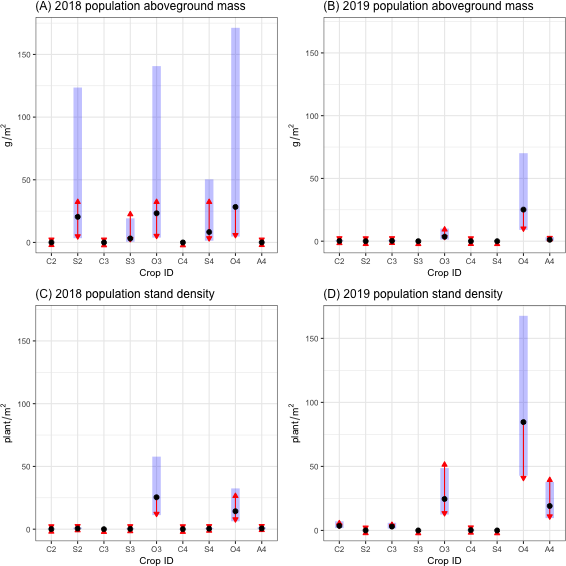
\includegraphics{Population-sex-biom-dens_files/figure-latex/pop-biom-dens-all-1.png}
\caption{\label{fig:pop-biom-dens-all}Waterhemp population aboveground mass and stand density averaged over corn weed managements. The abbreviations on the x-axis are crop identities, which are the combinations of the first letter in crop species names and the rotation to which the crops belonged (C2: corn in the 2-year rotation, C3: corn in the 3-year rotation, C4: corn in the 4-year rotation, S2: soybean in the 2-year rotation, S3: soybean in the 3-year rotation; S4: soybean in the 4-year rotation, O3: oat in the 3-year rotation, O4: oat in the 4-year rotation, and A4: alfalfa in the 4-year rotation). The black dots are estimated marginal means. The blue bars are 95\% confidence intervals. The red arrows reflect the comparison among means. Overlapping arrows indicate non-significant differences.}
\end{figure}

\begin{table}

\caption{\label{tab:pbiom-dens-ct}Rotation system and crop effects on population aboveground mass and stand density.}
\centering
\begin{threeparttable}
\begin{tabular}[t]{lrlr>{}l|rlrl}
\toprule
\multicolumn{1}{c}{ } & \multicolumn{4}{c}{2018} & \multicolumn{4}{c}{2019} \\
\cmidrule(l{3pt}r{3pt}){2-5} \cmidrule(l{3pt}r{3pt}){6-9}
\multicolumn{1}{c}{ } & \multicolumn{2}{c}{\makecell[c]{Population \\ aboveground mass}} & \multicolumn{2}{c}{\makecell[c]{Population \\ stand density}} & \multicolumn{2}{c}{\makecell[c]{Population \\ aboveground mass}} & \multicolumn{2}{c}{\makecell[c]{Population \\ stand density}} \\
\cmidrule(l{3pt}r{3pt}){2-3} \cmidrule(l{3pt}r{3pt}){4-5} \cmidrule(l{3pt}r{3pt}){6-7} \cmidrule(l{3pt}r{3pt}){8-9}
Contrast & ratio & p.value & ratio & p.value & ratio & p.value & ratio & p.value\\
\midrule
\addlinespace[0.3em]
\multicolumn{9}{l}{\textbf{(A) - Rotation system effects}}\\
\hspace{1em}C2 vs C3 & 12.54 & 0.1237 & 2.38 & 0.2990 & 0.84 & 0.9680 & 1.19 & 0.9284\\
\hspace{1em}C2 vs C4 & 23.12 & 0.0430 & 1.84 & 0.5435 & 10.61 & 0.0054 & 14.45 & <.0001\\
\hspace{1em}C3 vs C4 & 1.84 & 0.8798 & 0.78 & 0.8983 & 12.65 & 0.0026 & 12.11 & <.0001\\
\hspace{1em}S2 vs S3 & 6.42 & 0.3151 & 2.07 & 0.4258 & 6.27 & 0.0369 & 2.60 & 0.1265\\
\hspace{1em}S2 vs S4 & 2.45 & 0.7597 & 1.29 & 0.8976 & 6.27 & 0.0369 & 2.60 & 0.1265\\
\hspace{1em}S3 vs S4 & 0.38 & 0.7298 & 0.62 & 0.6963 & 1.00 & 1.0000 & 1.00 & 1.0000\\
\hspace{1em}O3 vs O4 & 0.82 & 0.8774 & 1.78 & 0.3235 & 0.14 & 0.0096 & 0.29 & 0.0132\\
\addlinespace[0.3em]
\multicolumn{9}{l}{\textbf{(B) - Crop species effects}}\\
\hspace{1em}oat vs soybean & 3.15 & 0.5040 & 47.18 & <.0001 & 2580.00 & <.0001 & 1330.00 & <.0001\\
\hspace{1em}oat vs corn & 5795.38 & <.0001 & 222.88 & <.0001 & 85.30 & <.0001 & 32.60 & <.0001\\
\hspace{1em}oat vs alfalfa & 831.33 & <.0001 & 29.84 & <.0001 & 8.34 & 0.0071 & 2.39 & 0.1712\\
\hspace{1em}soybean vs corn & 1840.55 & <.0001 & 4.72 & 0.0001 & 0.03 & <.0001 & 0.02 & <.0001\\
\hspace{1em}soybean vs alfalfa & 264.02 & <.0001 & 0.63 & 0.7660 & 0.00 & <.0001 & 0.00 & <.0001\\
\hspace{1em}corn vs alfalfa & 0.14 & 0.2509 & 0.13 & 0.0005 & 0.10 & 0.0014 & 0.07 & <.0001\\
\bottomrule
\end{tabular}
\begin{tablenotes}[para]
\item \textit{Note: } 
\item Some zero values are due to rounding. C2: corn in the 2-year rotation, C3: corn in the 3-year rotation, C4: corn in the 4-year rotation, S2: soybean in the 2-year rotation, S3: soybean in the 3-year rotation; S4: soybean in the 4-year rotation, O3: oat in the 3-year rotation, O4: oat in the 4-year rotation, and A4: alfalfa in the 4-year rotation
\end{tablenotes}
\end{threeparttable}
\end{table}

\hypertarget{population-sex-ratio}{%
\subsection*{Population sex ratio}\label{population-sex-ratio}}
\addcontentsline{toc}{subsection}{Population sex ratio}

Population stand density was included to improve the precision of estimates of population sex ratios (Table \ref{tab:sexr18-covar-jt}C versus \ref{tab:sexr18-covar-jt}A). The population sex ratio in 2018 differed significantly among treatments, at different population stand densities within each treatment (p-value = 0.0155, Table \ref{tab:sexr18-covar-jt} and Figure \ref{fig:sexr18-dens-arrow}). Therefore, sex ratios in the same treatment were evaluated at four population densities, i.e., 1, 5, 50, and 500 plants/m\(^2\), to illustrate that three-way interaction (Figure \ref{fig:sexr18-dens-arrow}). Female-biasedness was more likely if a waterhemp population was grown in oat and alfalfa. None of the waterhemp populations grown in corn and soybean expressed gender biasedness. It is unclear whether the corn weed management program had a significant effect on gender biasedness given the magnitude of the variance (Figure \ref{fig:sexr18-dens-arrow}).

We defined a useful imputed data set to be a set that resulted in fully estimable marginal means for sex ratio comparison across all treatments, which was achievable with non-zeros in female and male categories in at least one replication among the four blocks for the missing observations in the 2019 original sex data. Unlike the 2018 data, the sex ratio in 2019 was analyzed without the covariates because none of the covariates improved the goodness of fit for the analysis model. With m = 24, five imputed data sets were useful (Appendix B). The significance and influence of treatment factors and their interaction in the imputed data sets for waterhemp sex ratio in 2019 were consistent with those of the 2018 data (Figure \ref{fig:sexr19-arrow}). In 21 out of 24 sets, sex ratio in 2019 was affected by crop identity (Figure \ref{fig:sexr19-arrow}B and \ref{fig:sexr19-arrow}C). Female biasedness was observed in oat and alfalfa but not in corn and soybean (Figure \ref{fig:sexr19-arrow}A).

\begin{landscape}\begin{table}

\caption{\label{tab:sexr18-covar-jt}ANOVAs of crop identity, herbicide, and covariate effects on population sex ratio using 2018 data. With population aboveground mass covariate included (B), crop identity was the only influential factor on population sex ratio. With population stand density covariate included (C), sex ratio responded differently in each treatment and stand density combination.}
\centering
\resizebox{\linewidth}{!}{
\begin{tabular}[t]{lllrl}
\toprule
Source of variation & df1 & df2 & F.value & p.value\\
\midrule
\addlinespace[0.3em]
\multicolumn{5}{l}{\textbf{(A) no covariate. Residual deviance = 165.9, dispersion = 3.32.}}\\
\hspace{1em}Crop ID & 8 & Inf & 8.45 & <.0001\\
\hspace{1em}Corn weed management & 1 & Inf & 0.01 & 0.9317\\
\hspace{1em}Crop ID x Corn weed management & 8 & Inf & 0.46 & 0.8862\\
\addlinespace[0.3em]
\multicolumn{5}{l}{\textbf{(B) with population aboveground mass covariate. Residual deviance = 104.3, dispersion = 3.24.}}\\
\hspace{1em}Crop ID & 8 & Inf & 1.02 & 0.4155\\
\hspace{1em}Corn weed management & 1 & Inf & 0.00 & 0.9601\\
\hspace{1em}Population aboveground mass & 1 & Inf & 1.51 & 0.2198\\
\hspace{1em}Crop ID x Corn weed management & 8 & Inf & 0.71 & 0.6847\\
\hspace{1em}Crop ID x Population aboveground mass & 8 & Inf & 1.04 & 0.4038\\
\hspace{1em}Corn weed management x Population aboveground mass & 1 & Inf & 2.85 & 0.0916\\
\hspace{1em}Crop ID x Corn weed management x Population aboveground mass & 8 & Inf & 1.24 & 0.2713\\
\addlinespace[0.3em]
\multicolumn{5}{l}{\textbf{(C) with population stand density covariate. Residual deviance = 82.12, dispersion = 2.54.}}\\
\hspace{1em}Crop ID & 8 & Inf & 0.96 & 0.4679\\
\hspace{1em}Corn weed management & 1 & Inf & 0.93 & 0.3346\\
\hspace{1em}Population stand density & 1 & Inf & 2.46 & 0.1169\\
\hspace{1em}Crop ID x Corn weed management & 8 & Inf & 1.46 & 0.1675\\
\hspace{1em}Crop ID x Population stand density & 8 & Inf & 1.71 & 0.0896\\
\hspace{1em}Corn weed management x Population stand density & 1 & Inf & 5.16 & 0.0231\\
\hspace{1em}Crop ID x Corn weed management x Population stand density & 8 & Inf & 2.36 & 0.0155\\
\bottomrule
\end{tabular}}
\end{table}
\end{landscape}

\begin{figure}
\centering
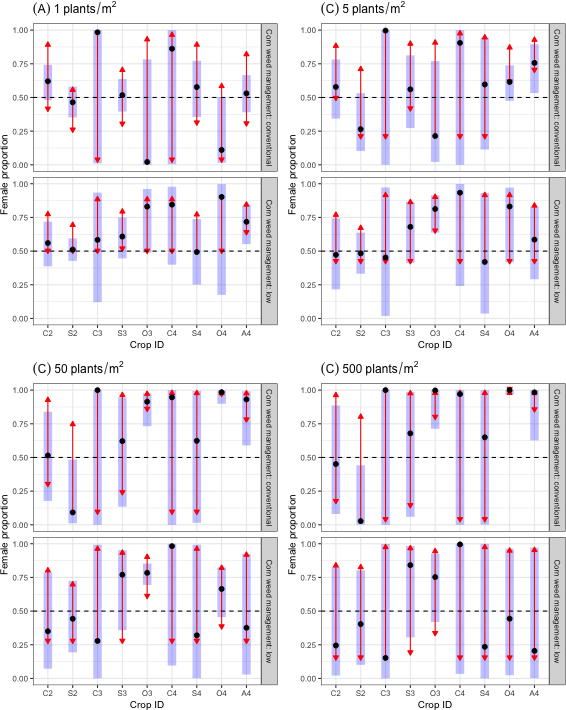
\includegraphics{Population-sex-biom-dens_files/figure-latex/sexr18-dens-arrow-1.png}
\caption{\label{fig:sexr18-dens-arrow}Waterhemp population sex ratios under 54 combinations of experimental treatments and population stand densities. The abbreviations on the x-axis are crop identities, which are the combinations of the first letter in crop species names and the rotation to which the crops belonged (C2: corn in the 2-year rotation, C3: corn in the 3-year rotation, C4: corn in the 4-year rotation, S2: soybean in the 2-year rotation, S3: soybean in the 3-year rotation; S4: soybean in the 4-year rotation, O3: oat in the 3-year rotation, O4: oat in the 4-year rotation, and A4: alfalfa in the 4-year rotation). The dashed lines mark sex ratio parity. The black dots are estimated marginal means. The blue bars are 95\% confidence intervals. The red arrows reflect the comparisons among means. Overlapping arrows indicate non-significant differences.}
\end{figure}

\begin{figure}
\centering
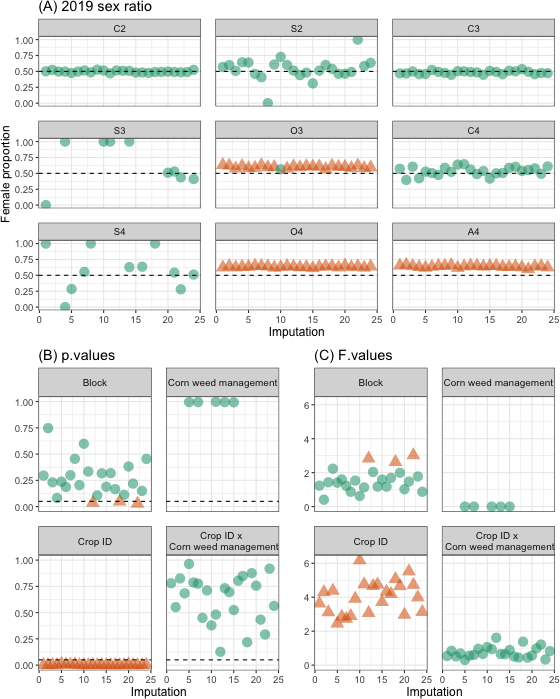
\includegraphics{Population-sex-biom-dens_files/figure-latex/sexr19-arrow-1.png}
\caption{\label{fig:sexr19-arrow}Waterhemp population sex ratios under nine crop idenitites averaged over two Corn weed management regimes using 2019's 24 imputed data sets (A). The dashed lines mark sex ratio parity in panel A and level of confidence in panel B, respectively. The blank spaces are nonestimable values. The triangulars and circles in panel A represent female-biased and even populations assessed at alpha = 0.05, respectively. F-values for sources of variation are shown in panel C.}
\end{figure}

\end{document}
